
%(BEGIN_QUESTION)
% Copyright 2010, Tony R. Kuphaldt, released under the Creative Commons Attribution License (v 1.0)
% This means you may do almost anything with this work of mine, so long as you give me proper credit

A water electrolyzer circuit converts AC power into DC, using a {\it shunt resistor} to help measure the amount of current passing through the electrolysis cells:

$$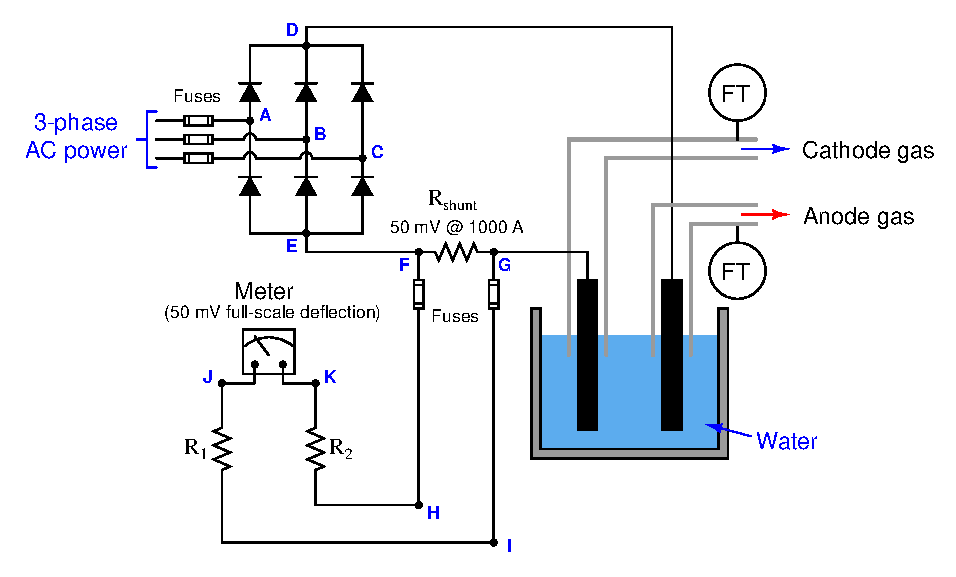
\includegraphics[width=15.5cm]{i00622x01.eps}$$

One day the operator for this electrolytic process calls you to say the gas production has suddenly stopped, yet the current meter indicates more than 1000 amps (the operator reports the meter are being ``pegged'' full-scale!).  Your first step is to measure voltage between points {\bf I} and {\bf H}, and there your multimeter shows far greater than 50 millivolts DC.

Identify the likelihood of each specified fault for this circuit.  Consider each fault one at a time (i.e. no coincidental faults), determining whether or not each fault could independently account for {\it all} measurements and symptoms in this circuit.

% No blank lines allowed between lines of an \halign structure!
% I use comments (%) instead, so that TeX doesn't choke.

$$\vbox{\offinterlineskip
\halign{\strut
\vrule \quad\hfil # \ \hfil & 
\vrule \quad\hfil # \ \hfil & 
\vrule \quad\hfil # \ \hfil \vrule \cr
\noalign{\hrule}
%
% First row
{\bf Fault} & {\bf Possible} & {\bf Impossible} \cr
%
\noalign{\hrule}
%
% Another row
$R_1$ or $R_2$ failed open &  &  \cr
%
\noalign{\hrule}
%
% Another row
$R_{shunt}$ failed open &  &  \cr
%
\noalign{\hrule}
%
% Another row
One meter fuse blown &  &  \cr
%
\noalign{\hrule}
%
% Another row
One AC power fuse blown &  &  \cr
%
\noalign{\hrule}
%
% Another row
$R_1$ or $R_2$ failed shorted &  &  \cr
%
\noalign{\hrule}
%
% Another row
$R_{shunt}$ failed shorted &  &  \cr
%
\noalign{\hrule}
%
% Another row
Open wire between G and cathode &  &  \cr
%
\noalign{\hrule}
%
% Another row
Open wire between D and anode &  &  \cr
%
\noalign{\hrule}
} % End of \halign 
}$$ % End of \vbox

Also, identify the gas types you would expect to find coming off the anode and cathode, respectively, and a good choice for flowmeter technologies to measure the flow of each gas.


\vfil

\underbar{file i00622}
\eject
%(END_QUESTION)





%(BEGIN_ANSWER)

This is a graded question -- no answers or hints given!

%(END_ANSWER)





%(BEGIN_NOTES)

If gas production has stopped, it definitely means the normal amount of current is no longer flowing through the electrolysis cell (i.e. the electric current has diminished greatly).  So, we are looking for any fault that could account for greatly diminished cell current while causing the ammeter to register higher than normal.  Of all the faults listed, there is only one capable of accounting for both these symptoms:

% No blank lines allowed between lines of an \halign structure!
% I use comments (%) instead, so that TeX doesn't choke.

$$\vbox{\offinterlineskip
\halign{\strut
\vrule \quad\hfil # \ \hfil & 
\vrule \quad\hfil # \ \hfil & 
\vrule \quad\hfil # \ \hfil \vrule \cr
\noalign{\hrule}
%
% First row
{\bf Fault} & {\bf Possible} & {\bf Impossible} \cr
%
\noalign{\hrule}
%
% Another row
$R_1$ or $R_2$ failed open &  & $\surd$ \cr
%
\noalign{\hrule}
%
% Another row
$R_{shunt}$ failed open & $\surd$ &  \cr
%
\noalign{\hrule}
%
% Another row
One meter fuse blown &  & $\surd$ \cr
%
\noalign{\hrule}
%
% Another row
One AC power fuse blown &  & $\surd$ \cr
%
\noalign{\hrule}
%
% Another row
$R_1$ or $R_2$ failed shorted &  & $\surd$ \cr
%
\noalign{\hrule}
%
% Another row
$R_{shunt}$ failed shorted &  & $\surd$ \cr
%
\noalign{\hrule}
%
% Another row
Open wire between G and cathode &  & $\surd$ \cr
%
\noalign{\hrule}
%
% Another row
Open wire between D and anode &  & $\surd$ \cr
%
\noalign{\hrule}
} % End of \halign 
}$$ % End of \vbox

Hydrogen gas will be found at the cathode, and oxygen gas at the anode.  A good type of flowmeter for each gas would be {\it thermal mass}: this type would yield measurements of true mass flow at low cost, with very little chance of measurement error due to changes in gas composition.

\vskip 20pt \vbox{\hrule \hbox{\strut \vrule{} {\bf Virtual Troubleshooting} \vrule} \hrule}

This question is a good candidate for a ``Virtual Troubleshooting'' exercise.  Presenting the diagram to students, you first imagine in your own mind a particular fault in the system.  Then, you present one or more symptoms of that fault (something noticeable by an operator or other user of the system).  Students then propose various diagnostic tests to perform on this system to identify the nature and location of the fault, as though they were technicians trying to troubleshoot the problem.  Your job is to tell them what the result(s) would be for each of the proposed diagnostic tests, documenting those results where all the students can see.

During and after the exercise, it is good to ask students follow-up questions such as:

\begin{itemize}
\item{} What does the result of the last diagnostic test tell you about the fault?
\item{} Suppose the results of the last diagnostic test were different.  What then would that result tell you about the fault?
\item{} Is the last diagnostic test the best one we could do?
\item{} What would be the ideal order of tests, to diagnose the problem in as few steps as possible?
\end{itemize}

%INDEX% Process: electrolysis of water
%INDEX% Troubleshooting review: electric circuits

%(END_NOTES)


